\documentclass{article}
\usepackage{graphicx}
\usepackage{amssymb,amsmath}
\usepackage{tikz}
\usepackage{pgfplots}
\pgfplotsset{compat=newest}
\pgfplotsset{plot coordinates/math parser=false}
\newlength\figureheight
\newlength\figurewidth
\usetikzlibrary{shapes, arrows, patterns, external}

\DeclareRobustCommand{\BlackBox}{\State \textbf{Black Box: }}
\DeclareRobustCommand{\Test}{\State \textbf{Test: }}
\DeclareRobustCommand{\Define}{\State \textbf{Define: }}
\DeclareRobustCommand{\Update}{\State \textbf{Update: }}
\DeclareRobustCommand{\Set}{\State \textbf{Set: }}
\DeclareRobustCommand{\Calculate}{\State \textbf{Calculate: }}
%\newcommand{\algorithmicset}{\textbf{Set:}}
%\algnewcommand\Solve{\item[\algorithmicset]}
%============================================================================
% commands.tex
%============================================================================
% This file contains:
% 	- Defined Variables
%	- Redefined math shorthand
%	- Defined math shorthand

%============================================================================
% Defined Variables
%============================================================================
% 	- \abstractType:
%		Use: Toggles the type of abstract to be used
%		Default Value: abstract
%		Options: abstract, umiabstract
\newcommand{\abstractType}{abstract}

%============================================================================
% Redefined Math Commands
%============================================================================
% 	- \Vec{1} or \vec{1}
%		Long Name: Vector
%		Arguements[1]: bold and overbar arg1	
\DeclareRobustCommand{\Vec}[1]{%
    \ifmmode
        \mathbf{#1}\,%
    \else
        $\displaystyle \mathbf{#1}\,$%
    \fi
}
\DeclareRobustCommand{\vec}[1]{\Vec{#1}}

\DeclareRobustCommand{\lbm}{%
    \ifmmode
        \text{lb}_{\text{m}}
    \else
        $\displaystyle \text{lb}_{\text{m}}$%
    \fi
}
\DeclareRobustCommand{\lbf}{%
    \ifmmode
        \text{lb}_{\text{f}}
    \else
        $\displaystyle \text{lb}_{\text{f}}$
    \fi
}
\DeclareRobustCommand{\dt}{%
	\ifmmode
		\Delta t
	\else
		$Delta t$
	\fi
}
\DeclareRobustCommand{\dtmax}{%
	\ifmmode
		\Delta t_{\text{MAX}}
	\else
		$\Delta t_{\text{MAX}}$
	\fi
}
\DeclareRobustCommand{\dx}{%
	\ifmmode
		\Delta x
	\else
		$\Delta x$
	\fi
}

\delimitershortfall-1sp
\newcommand\abs[1]{\left|#1\right|}

\tikzstyle{Decision} = [diamond, draw, text width=4.5em, text badly centered, node distance=3cm, inner sep=0pt]
\tikzstyle{Action} = [rectangle, draw,text width=5em, text centered, node distance=3cm, rounded corners, minimum height=0em]
\tikzstyle{NodePoint} = [circle, draw, minimum height = 0 em, node distance = 3 cm]
\tikzstyle{BlackBox} = [rectangle, draw, text centered, node distance=1cm, fill=black!10]
\tikzstyle{line} = [draw, -latex']
    

\begin{document}
\begin{figure}
\centering
\begin{center}
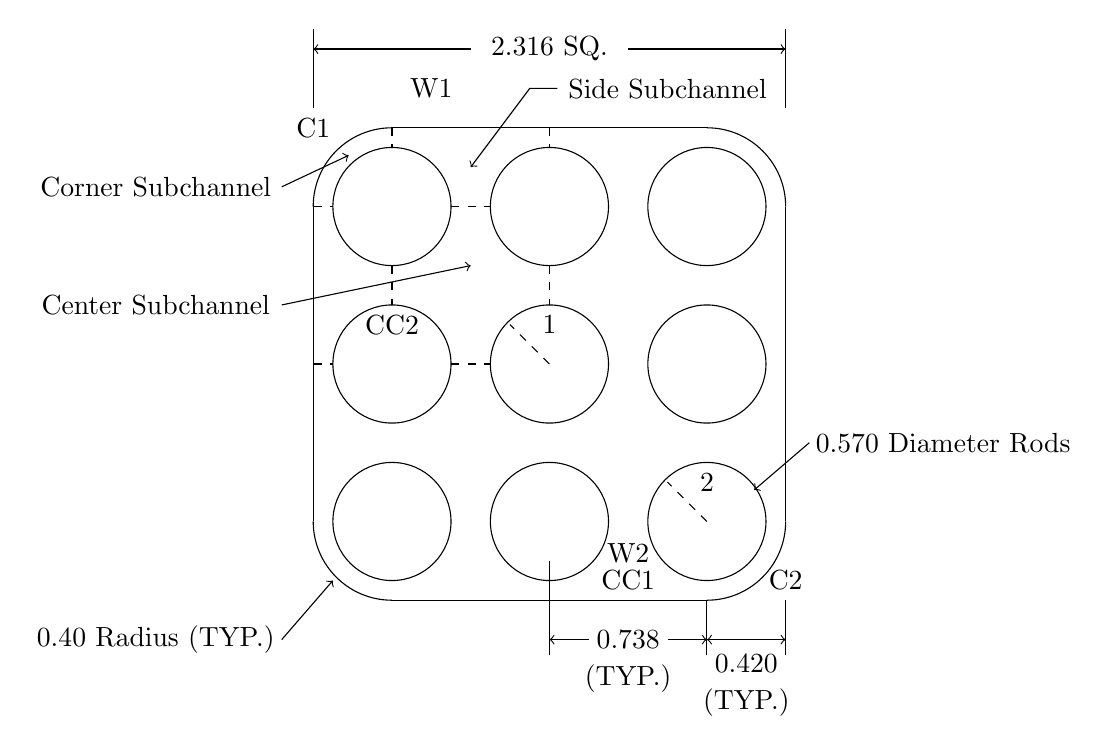
\begin{tikzpicture}

%Rounded corners
\draw (3,2) arc (0:90:1);
\draw (-2,3) arc (90:180:1);
\draw (-3,-2) arc (180:270:1);
\draw (2,-3) arc (270:360:1);

%Grid of circles
\draw (0,0) circle (0.75);
\draw (0,2) circle (0.75);
\draw (0,-2) circle (0.75);
\draw (2,0) circle (0.75);
\draw (2,2) circle (0.75);
\draw (2,-2) circle (0.75);
\draw (-2,0) circle (0.75);
\draw (-2,2) circle (0.75);
\draw (-2,-2) circle (0.75);

%Box
\draw (-3,-2) -- (-3,2);
\draw (3,-2) -- (3,2);
\draw (2,-3) -- (-2,-3);
\draw (-2,3) -- (2,3);

%Misc lines
\draw [dashed] (-2,3) -- (-2,2.75);
\draw [dashed] (0,3) -- (0,2.75);
\draw [dashed] (-2,1.25) -- (-2,0.75);
\draw [dashed] (0,1.25) -- (0,0.75);
\draw [dashed] (-3,2) -- (-2.75,2);
\draw [dashed] (-3,0) -- (-2.75,0);
\draw [dashed] (-1.25,2) -- (-0.75,2);
\draw [dashed] (-1.25,0) -- (-0.75,0);

\draw [dashed] (0,0) -- (-0.5,0.5);
\draw [dashed] (2,-2) -- (1.5,-1.5);

%Misc arrows and labels
\draw [<-] (-3,4) -- (-1,4);
\draw [->] (1,4) -- (3,4);
\draw (-3,4.25) -- (-3,3.25);
\draw (3,4.25) -- (3,3.25);
\draw (0,4) node {2.316 SQ.};

\draw [<-] (0,-3.5) -- (0.5,-3.5);
\draw [->] (1.5,-3.5) -- (2,-3.5);
\draw (2,-3.7) -- (2,-3);
\draw (0,-3.7) -- (0,-2.5);
\draw (1,-3.5) node {0.738};
\draw (1,-4) node {(TYP.)};

\draw [<->] (2,-3.5) -- (3,-3.5);
\draw (3,-3.7) -- (3,-3);
\draw (2.5,-3.8) node {0.420};
\draw (2.5,-4.3) node {(TYP.)};

\draw [->] (-3.4,2.25) -- (-2.55,2.65);
\draw (-5,2.25) node {Corner Subchannel};

\draw [->] (-3.4,0.75) -- (-1,1.25);
\draw (-5,0.75) node {Center Subchannel};

\draw [->] (0.1,3.5) -- (-0.25,3.5) -- (-1,2.5);
\draw (1.5,3.5) node {Side Subchannel};

\draw [->] (-3.4,-3.5) -- (-2.75,-2.75);
\draw (-5,-3.5) node {0.40 Radius (TYP.)};

\draw [->] (3.3,-1) -- (2.6,-1.6);
\draw (5,-1) node {0.570 Diameter Rods};

\draw (-3,3) node {C1};
\draw (-1.5,3.5) node {W1};
\draw (1,-2.75) node {CC1};

\draw (3,-2.75) node {C2};
\draw (1,-2.4) node {W2};
\draw (-2,0.5) node {CC2};

\draw (0,0.5) node {1};
\draw (2,-1.5) node {2};

\end{tikzpicture}
\end{center}
\caption{Position of pressure taps for setting isokinetic conditions. Note splitter positions for the various subchannels.}
\label{fig:position_of_pressure taps}
\end{figure}

\end{document}